% TODO criteria about how to "rate" approaches

\section{Ontology 101}

\section{Methodology by Noy and McGuinness}

\section{Methodology by Uschold and King}

\section{Methodology by Grüninger and Fox}

\section{METHONTOLOGY}

% TODO mention IEEE software life cycle paper referenced in \cite{MethontologyLegal}?
The authors of the article introducing the approach named \methontology, Gómez-Pérez et al., perceived absence of a clear engineering approach towards building ontology from scratch \cite{Methontology}. Hence, Gómez-Pérez et al. described a process for developing ontologies and specified a life cycle for ontologies. Based upon that, they specified \methontology as a straight-forward engineering approach for building ontologies.

% TODO reference more papers?
There are several papers describing how to apply \methontology on certain domains \cite{MethontologyLegal} \cite{MethontologyChemical}. While the overall approach is the same in all of these articles, there are slight differences in the details of each step. This section describes the steps used in chapter \ref{ch:thinkhomeweather_ontology}. Thus, it differs slightly from the steps described in \cite{Methontology}.

\subsection{Ontology development process and life cycle}

The ontology development process as used by Gómez-Pérez et al. divides ontology development into the following activities that need to be performed \cite{Methontology}:

% TODO emphazise steps as in \cite{Methontology}?
% TODO remove 'must's
\begin{itemize}
  \item The whole process must be planned regarding which tasks need to be done, how they will be arranged and which resources they require.
  \item The purpose, intended uses and end-users must be specified in an ontologies requirements specification document.
  \item Knowledge about the ontology's domain must be acquired.
  \item The knowledge previously acquired must be conceptualized in a conceptual model describing the problem and its solution.
  \item This conceptual model will then be formalized.
  \item As ontologies are build to be reused, as many existing ontologies as possible will be integrated into the new ontology.
  \item The ontology will then be implemented using a formal language.
  \item The implemented ontology will be evaluated in order to ensure it fits the requirements specified previously.
  \item The whole work must be documented well.
  \item There are always things that can be modified in an ontology, therefore maintenance is necessary.
\end{itemize}

\begin{figure}[]
  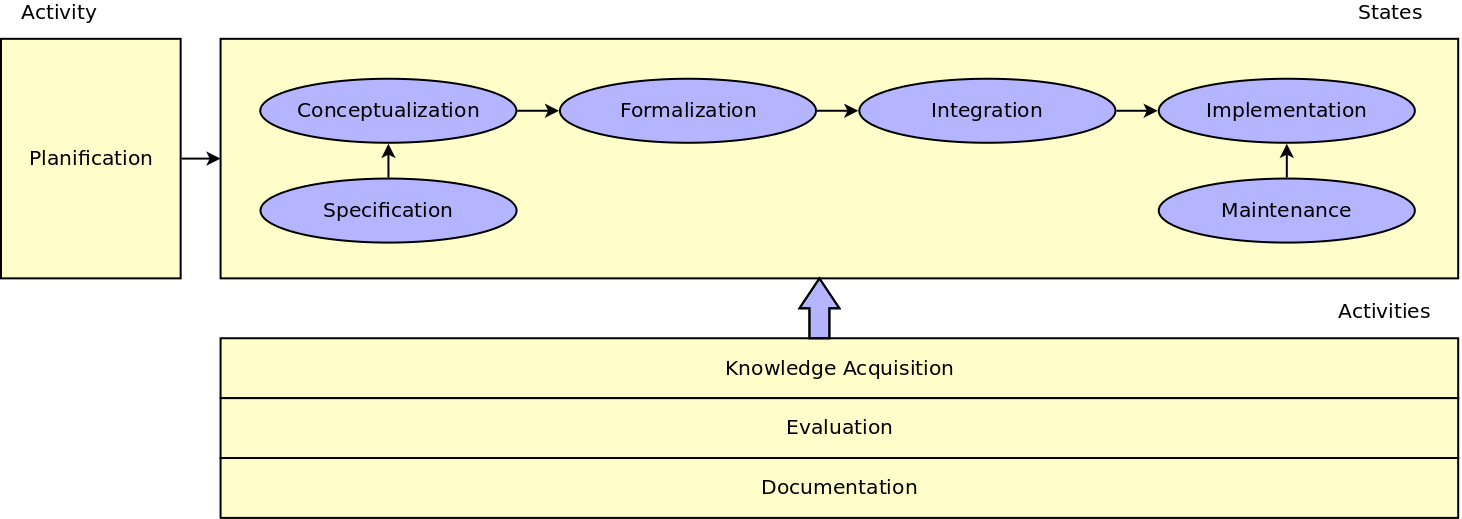
\includegraphics[width=\textwidth]{figures/ontology_lifecycle.png}
  \caption{States and activities in the life cycle of an ontology according to \methontology \cite{Methontology}}
\end{figure}

As seen in figure \ref{fig:methontology1}, these groups are split into \emph{planification} that must be performed at the very beginning of development, a \emph{set of stages} (consisting of \emph{specification}, \emph{conceptualization}, \emph{formalization}, \emph{integration}, \emph{implementation} and \emph{maintenance}) through which the ontology moves during its life and some activities (\emph{knowledge acquisition}, \emph{documentation} and \emph{evaluation}) that are performed during the whole development process in parallel to the stages.

Differently to what is shown in figure \ref{fig:methontology1}, \methontology follows an \emph{evolving} life cycle model which allows the ontology to grow according to its needs. Whenever it is necessary, pieces of the ontology can be added, modified and deleted. Thus, one state does not have to be completely finished before the next state is begun. The ontology will cycle through each state numerous times until the ontology fits the requirements and the results of each step correspond to each other.

\subsection{METHONTOLOGY}

\subsubsection{Specification}


\subsubsection{Knowledge Acquisition}

\subsubsection{Conceptualization}

\paragraph{Glossary of Terms}

\paragraph{Concept Taxonomies}

\paragraph{Ad-hoc binary relation diagrams}

\paragraph{Concept dictionary}

\paragraph{Ad-hoc binary relation details}

\paragraph{Instance attributes}

\paragraph{Class attributes}

\paragraph{Constants}

\paragraph{Formal axioms}

\paragraph{Rules}

\paragraph{Instances}


\subsubsection{Integration}

\subsubsection{Implementation}

\subsubsection{Evaluation}

\subsubsection{Documentation}

\section{Software engineering approach by De Nicola, Missikoff and Navigli}

\section{Conclusion}

The previous chapters gave detailled insights into some popular approaches of developing ontologies from scratch. Table ? summarizes some of the key charasteristics of these approaches.

% TODO insert table

Considering the characteristics of the development approaches, \methontology was chosen for building the \thinkhomeweather ontology. Thus, \methontology was discussed more thoroughly than the other approaches. The main reasons for that decision were:

% TODO
\begin{itemize}
  \item Some reason.
  \item Some more reason.
  \item And yet another reason.
\end{itemize}

Chapter \ref{ch:thinkhomeweather_ontology} describes the process of building the \thinkhomeweather ontology in detail.